\input format.tex

\usepackage{graphicx}
\graphicspath{{cores/}}

\usepackage{environ}
\usepackage{colortbl,array,booktabs}
\usepackage{tabularx}

\colorlet{TablaBordeSuperior}{topcolor}
\colorlet{TablaBordeInferior}{topcolor}
\colorlet{TablaCentroSuperior}{blue!1}
\colorlet{TablaCentroInferior}{blue!20}
\colorlet{FuenteCabeceraTabla}{white}

\newcolumntype{M}[1]{>{\centering\arraybackslash}m{#1}}
%\newcommand{\tabularxcolumn}[1]{>\arraybackslash}m{#1}}

\tcbset{rtab/.style={
freelance,
frame code={
 \path[top color=topcolor,bottom color=topcolor]
   ([yshift=-#1*(\baselineskip+2pt)]interior.north west) --
   ([yshift=-#1*(\baselineskip+2pt)]interior.north east) {[sharp corners]--
    ([yshift=3pt]interior.north east) --
    ([yshift=3pt]interior.north west)} -- cycle;

  },
interior code={},
 }
}

\newcommand\fuentecabecera[1]{\textcolor{black}{\textbf{#1}}}

\begin{document}

\vspace*{3mm}
%% 各章节
\setlength{\arrayrulewidth}{.2pt}
\fontsize{8.8pt}{11pt}\selectfont
\color{gray2}

\noindent{\bf{胖菌与瘦菌}}


\begin{spacing}{1.5}
\begin{LRaside}[.8]{\fontsize{8.8pt}{11pt}\selectfont 检测说明}
\noindent
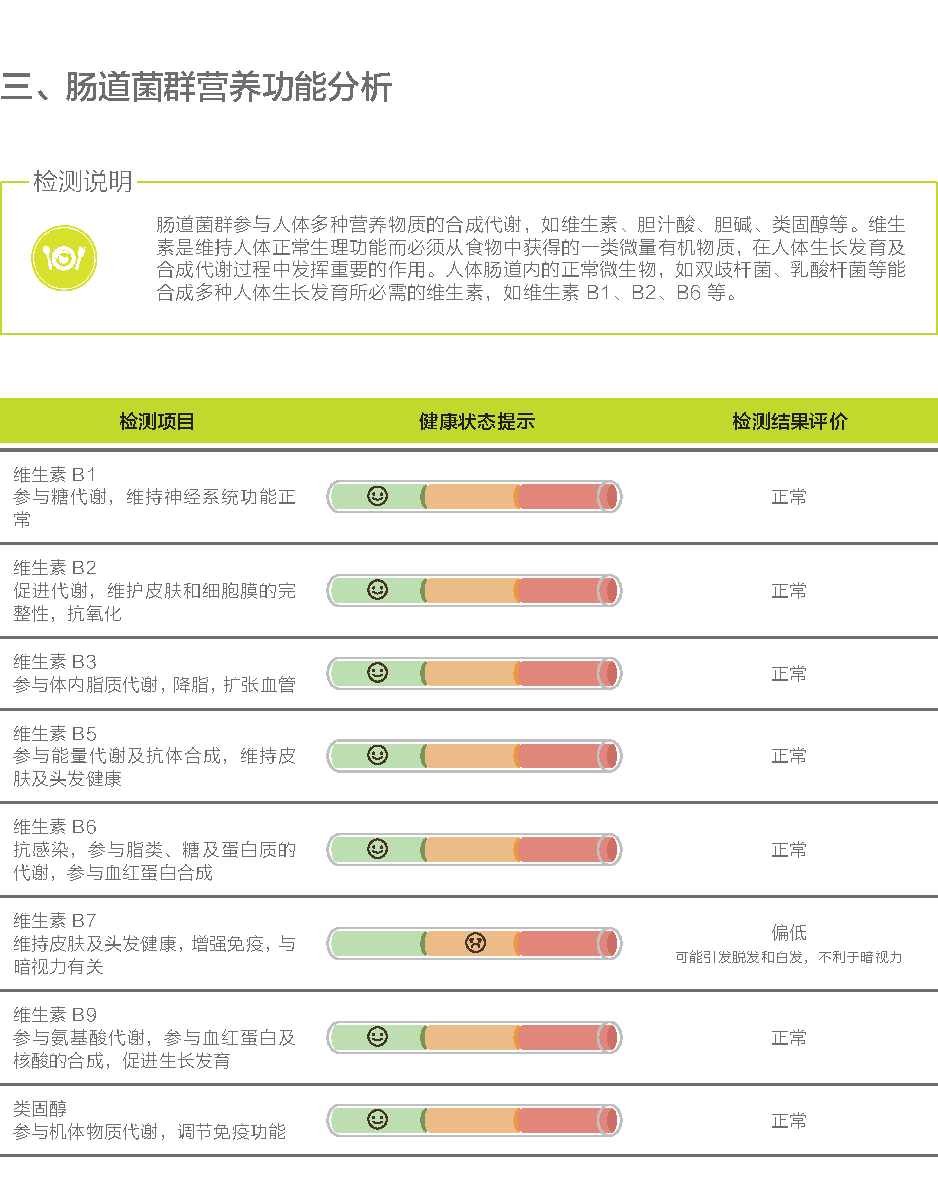
\includegraphics[width=\linewidth]{yingyanggongneng.pdf}
\asidebreak %
%{\fontsize{8pt}{11pt}\selectfont 常有人抱怨喝水都长胖,羡慕瘦子怎么都吃不胖,其实长胖很大可能是肠道菌群在捣鬼,其中肠道微生态中有两类菌是脱不了关系的,它们含量的高低决定了是否属
%于易胖体质,直接影响减重的难易程度。一类是增重肠道菌(简称胖菌),与肥胖成正相关,含量越高,肥胖程度越重,减肥难度越高,且易引起代谢综合症等疾病,影响
%人体健康;第二类是减重肠道菌(简称瘦菌),与肥胖成负相关,含量越少,越易肥胖,且肥胖程度与症状越重。因此通过检测,能够精准地找到引起肥胖的异常胖菌或瘦
%菌的种类/含量,有助于个性化减重,预防肥胖的发生。}
{\fontsize{8pt}{11pt}\selectfont 最新研究发现,肠道中有两类细菌与人体的肥胖密切相关,它们含量的高低不仅决定了是否属于易胖体质,而且对减重的难易程度有直接的影响。一类是引起肥胖的肠道
菌株(简称胖菌),与肥胖成正相关,其含量越高,肥胖程度越重,减肥难度越大,且易引起代谢综合症等疾病,影响人体健康;第二类是与减重相关的肠道菌株(简称瘦菌),与肥胖成负相关,其含量越
少,越易肥胖,且肥胖程度与症状越重。因此通过肠道菌群检测,精准检测出与肥胖相关的胖菌或瘦菌的种类以及含量,不仅有助于科学、个性化减重,且对肥胖的发生有积极的预防作用。}
\end{LRaside}
\end{spacing}

\noindent 检测结果

\hfill {\bf {肥胖菌总量 \quad}
{\color{green3}偏低}
}


\begin{tctabularx}{tabularx={m{4cm}<{\centering}m{6.6cm}<{\centering}m{4cm}<{\centering}}}
&&
\\[-6pt]
\cellcolor{topcolor} \raisebox{2.614pt}{\color{gray0}\bf 检测项目} &
\cellcolor{topcolor} \raisebox{2.614pt}{\color{gray0}\bf 健康状态提示} &
\cellcolor{topcolor} \raisebox{2.614pt}{\color{gray0}\bf 检测结果评价}
\end{tctabularx}

\vspace*{-4.25mm}
\fontsize{8pt}{11pt}\selectfont
\arrayrulecolor{gray2}
\begin{longtable}{m{4cm}<{\centering}m{6.6cm}<{\centering}m{4cm}<{\centering}}
\hline
%\parbox[c]{\hsize}{\vskip7pt {\lantxh 肠杆菌属\\ \bahao HASH(0x279ead8)} \vskip7pt} 
\parbox[c]{\hsize}{\vskip7pt {\lantxh 肠杆菌属} \vskip7pt}
& \parbox[c]{\hsize}{\vskip7pt\centerline{\raisebox{-1.5ex}{
\includegraphics[width=6cm,height=0.55cm]{pangjun-l2.pdf}}}\vskip7pt} &
\begin{minipage}{4cm}\begin{center}{{\lantxh 偏低} }\end{center} \end{minipage} \\
\hline
%\parbox[c]{\hsize}{\vskip7pt {\lantxh 梭菌属\\ \bahao 多数为致病菌,可能引起腹泻、肠炎等疾病} \vskip7pt} 
\parbox[c]{\hsize}{\vskip7pt {\lantxh 梭菌属} \vskip7pt}
& \parbox[c]{\hsize}{\vskip7pt\centerline{\raisebox{-1.5ex}{
\includegraphics[width=6cm,height=0.55cm]{pangjun-l2.pdf}}}\vskip7pt} &
\begin{minipage}{4cm}\begin{center}{{\lantxh 偏低} }\end{center} \end{minipage} \\
\hline
%\parbox[c]{\hsize}{\vskip7pt {\lantxh 布劳特氏菌属\\ \bahao 发酵多种植物多糖产生乙酸盐,促进肠道健康} \vskip7pt} 
\parbox[c]{\hsize}{\vskip7pt {\lantxh 布劳特氏菌属} \vskip7pt}
& \parbox[c]{\hsize}{\vskip7pt\centerline{\raisebox{-1.5ex}{
\includegraphics[width=6cm,height=0.55cm]{pangjun-l2.pdf}}}\vskip7pt} &
\begin{minipage}{4cm}\begin{center}{{\lantxh 偏低} }\end{center} \end{minipage} \\
\hline
%\parbox[c]{\hsize}{\vskip7pt {\lantxh 多尔氏菌属\\ \bahao 肠道的主要产气菌之一,与肠易激综合征等疾病相关} \vskip7pt} 
\parbox[c]{\hsize}{\vskip7pt {\lantxh 多尔氏菌属} \vskip7pt}
& \parbox[c]{\hsize}{\vskip7pt\centerline{\raisebox{-1.5ex}{
\includegraphics[width=6cm,height=0.55cm]{pangjun-l2.pdf}}}\vskip7pt} &
\begin{minipage}{4cm}\begin{center}{{\lantxh 偏低} }\end{center} \end{minipage} \\
\hline
%\parbox[c]{\hsize}{\vskip7pt {\lantxh 沙门氏菌属\\ \bahao HASH(0x279f258)} \vskip7pt} 
\parbox[c]{\hsize}{\vskip7pt {\lantxh 沙门氏菌属} \vskip7pt}
& \parbox[c]{\hsize}{\vskip7pt\centerline{\raisebox{-1.5ex}{
\includegraphics[width=6cm,height=0.55cm]{pangjun-l2.pdf}}}\vskip7pt} &
\begin{minipage}{4cm}\begin{center}{{\lantxh 偏低} }\end{center} \end{minipage} \\
\hline
%\parbox[c]{\hsize}{\vskip7pt {\lantxh 弯曲杆菌属\\ \bahao 多数菌种为致病菌,可引起弯曲菌病,表现为严重腹泻或痢疾综合征} \vskip7pt} 
\parbox[c]{\hsize}{\vskip7pt {\lantxh 弯曲杆菌属} \vskip7pt}
& \parbox[c]{\hsize}{\vskip7pt\centerline{\raisebox{-1.5ex}{
\includegraphics[width=6cm,height=0.55cm]{pangjun-l4.pdf}}}\vskip7pt} &
\begin{minipage}{4cm}\begin{center}{{\lantxh 偏高} }\end{center} \end{minipage} \\
\hline
%\parbox[c]{\hsize}{\vskip7pt {\lantxh 志贺氏菌属\\ \bahao HASH(0x27a1060)} \vskip7pt} 
\parbox[c]{\hsize}{\vskip7pt {\lantxh 志贺氏菌属} \vskip7pt}
& \parbox[c]{\hsize}{\vskip7pt\centerline{\raisebox{-1.5ex}{
\includegraphics[width=6cm,height=0.55cm]{pangjun-l2.pdf}}}\vskip7pt} &
\begin{minipage}{4cm}\begin{center}{{\lantxh 偏低} }\end{center} \end{minipage} \\
\hline
%\parbox[c]{\hsize}{\vskip7pt {\lantxh 克雷伯氏菌属\\ \bahao 多为致病菌,可能导致肺炎、尿路感染、软组织感染、菌血症等} \vskip7pt} 
\parbox[c]{\hsize}{\vskip7pt {\lantxh 克雷伯氏菌属} \vskip7pt}
& \parbox[c]{\hsize}{\vskip7pt\centerline{\raisebox{-1.5ex}{
\includegraphics[width=6cm,height=0.55cm]{pangjun-l2.pdf}}}\vskip7pt} &
\begin{minipage}{4cm}\begin{center}{{\lantxh 偏低} }\end{center} \end{minipage} \\
\hline
%\parbox[c]{\hsize}{\vskip7pt {\lantxh 脱硫弧菌属\\ \bahao 产生硫化氢,刺激肠道产生炎症反应,不利于肠道健康} \vskip7pt} 
\parbox[c]{\hsize}{\vskip7pt {\lantxh 脱硫弧菌属} \vskip7pt}
& \parbox[c]{\hsize}{\vskip7pt\centerline{\raisebox{-1.5ex}{
\includegraphics[width=6cm,height=0.55cm]{pangjun-l4.pdf}}}\vskip7pt} &
\begin{minipage}{4cm}\begin{center}{{\lantxh 偏高} }\end{center} \end{minipage} \\
\hline
%\parbox[c]{\hsize}{\vskip7pt {\lantxh 嗜胆菌属\\ \bahao 共生菌,可能与长期高脂高蛋白饮食有关} \vskip7pt} 
\parbox[c]{\hsize}{\vskip7pt {\lantxh 嗜胆菌属} \vskip7pt}
& \parbox[c]{\hsize}{\vskip7pt\centerline{\raisebox{-1.5ex}{
\includegraphics[width=6cm,height=0.55cm]{pangjun-l3.pdf}}}\vskip7pt} &
\begin{minipage}{4cm}\begin{center}{{\lantxh 正常} }\end{center} \end{minipage} \\
\hline
\end{longtable}

\clearpage

\vspace*{8mm}
%% 各章节
\setlength{\arrayrulewidth}{.2pt}
\fontsize{8.8pt}{11pt}\selectfont
\color{gray2}

\hfill {\bf {瘦菌总量 \quad}
{\color{orange2}偏低}
}

\begin{tctabularx}{tabularx={m{4cm}<{\centering}m{6.6cm}<{\centering}m{4cm}<{\centering}}}
&&
\\[-6pt]
\cellcolor{topcolor} \raisebox{2.614pt}{\color{gray0}\bf 检测项目} &
\cellcolor{topcolor} \raisebox{2.614pt}{\color{gray0}\bf 健康状态提示} &
\cellcolor{topcolor} \raisebox{2.614pt}{\color{gray0}\bf 检测结果评价}
\end{tctabularx}

\vspace*{-4.25mm}
\fontsize{8pt}{11pt}\selectfont
\arrayrulecolor{gray2}
\begin{longtable}{m{4cm}<{\centering}m{6.6cm}<{\centering}m{4cm}<{\centering}}
\hline
%\parbox[c]{\hsize}{\vskip7pt {\lantxh 阿克曼氏菌属\\ \bahao 降解粘蛋白、调节免疫,有利于肠黏膜完整性,保持正常体重} \vskip7pt} 
\parbox[c]{\hsize}{\vskip7pt {\lantxh 阿克曼氏菌属} \vskip7pt}
& \parbox[c]{\hsize}{\vskip7pt\centerline{\raisebox{-1.5ex}{
\includegraphics[width=6cm,height=0.55cm]{shoujun-l3.pdf}}}\vskip7pt} &
\begin{minipage}{4cm}\begin{center}{{\lantxh 正常} }\end{center} \end{minipage} \\
\hline
%\parbox[c]{\hsize}{\vskip7pt {\lantxh 双歧杆菌属\\ \bahao 有益菌,降解人体不能消化的多糖,产乳酸,调节免疫及肠道环境} \vskip7pt} 
\parbox[c]{\hsize}{\vskip7pt {\lantxh 双歧杆菌属} \vskip7pt}
& \parbox[c]{\hsize}{\vskip7pt\centerline{\raisebox{-1.5ex}{
\includegraphics[width=6cm,height=0.55cm]{shoujun-l2.pdf}}}\vskip7pt} &
\begin{minipage}{4cm}\begin{center}{{\lantxh 偏低} }\end{center} \end{minipage} \\
\hline
%\parbox[c]{\hsize}{\vskip7pt {\lantxh 乳酸杆菌属\\ \bahao 肠道益生菌,能够生成乳酸,抑制有害菌及炎症,调节肠道环境} \vskip7pt} 
\parbox[c]{\hsize}{\vskip7pt {\lantxh 乳酸杆菌属} \vskip7pt}
& \parbox[c]{\hsize}{\vskip7pt\centerline{\raisebox{-1.5ex}{
\includegraphics[width=6cm,height=0.55cm]{shoujun-l2.pdf}}}\vskip7pt} &
\begin{minipage}{4cm}\begin{center}{{\lantxh 偏低} }\end{center} \end{minipage} \\
\hline
%\parbox[c]{\hsize}{\vskip7pt {\lantxh 克里斯滕森菌属\\ \bahao HASH(0x27f21a0)} \vskip7pt} 
\parbox[c]{\hsize}{\vskip7pt {\lantxh 克里斯滕森菌属} \vskip7pt}
& \parbox[c]{\hsize}{\vskip7pt\centerline{\raisebox{-1.5ex}{
\includegraphics[width=6cm,height=0.55cm]{shoujun-l2.pdf}}}\vskip7pt} &
\begin{minipage}{4cm}\begin{center}{{\lantxh 偏低} }\end{center} \end{minipage} \\
\hline
%\parbox[c]{\hsize}{\vskip7pt {\lantxh 柔嫩梭菌属\\ \bahao 发酵纤维素产生丁酸等有益物质,抑制肠道炎症,促进肠道健康} \vskip7pt} 
\parbox[c]{\hsize}{\vskip7pt {\lantxh 柔嫩梭菌属} \vskip7pt}
& \parbox[c]{\hsize}{\vskip7pt\centerline{\raisebox{-1.5ex}{
\includegraphics[width=6cm,height=0.55cm]{shoujun-l2.pdf}}}\vskip7pt} &
\begin{minipage}{4cm}\begin{center}{{\lantxh 偏低} }\end{center} \end{minipage} \\
\hline
%\parbox[c]{\hsize}{\vskip7pt {\lantxh 颤螺菌属\\ \bahao 帮助抗性淀粉和脂肪消化,保持正常体重,抑制肠道炎症} \vskip7pt} 
\parbox[c]{\hsize}{\vskip7pt {\lantxh 颤螺菌属} \vskip7pt}
& \parbox[c]{\hsize}{\vskip7pt\centerline{\raisebox{-1.5ex}{
\includegraphics[width=6cm,height=0.55cm]{shoujun-l3.pdf}}}\vskip7pt} &
\begin{minipage}{4cm}\begin{center}{{\lantxh 正常} }\end{center} \end{minipage} \\
\hline
%\parbox[c]{\hsize}{\vskip7pt {\lantxh 毛螺菌属\\ \bahao 发酵多种糖类产生乙酸、甲酸等物质,能保护肠黏膜,抑制肠道炎症} \vskip7pt} 
\parbox[c]{\hsize}{\vskip7pt {\lantxh 毛螺菌属} \vskip7pt}
& \parbox[c]{\hsize}{\vskip7pt\centerline{\raisebox{-1.5ex}{
\includegraphics[width=6cm,height=0.55cm]{shoujun-l4.pdf}}}\vskip7pt} &
\begin{minipage}{4cm}\begin{center}{{\lantxh 偏高} }\end{center} \end{minipage} \\
\hline
%\parbox[c]{\hsize}{\vskip7pt {\lantxh 毛杆菌属\\ \bahao 肠道共生菌,发酵葡萄糖产生乳酸及少量乙酸和丁酸} \vskip7pt} 
\parbox[c]{\hsize}{\vskip7pt {\lantxh 毛杆菌属} \vskip7pt}
& \parbox[c]{\hsize}{\vskip7pt\centerline{\raisebox{-1.5ex}{
\includegraphics[width=6cm,height=0.55cm]{shoujun-l2.pdf}}}\vskip7pt} &
\begin{minipage}{4cm}\begin{center}{{\lantxh 偏低} }\end{center} \end{minipage} \\
\hline
\end{longtable}

\vspace*{3mm}

\begin{spacing}{1.5}
\begin{LRaside}[.8]{\fontsize{8.8pt}{11pt}\selectfont 结果分析}
\noindent

\includegraphics[width=\linewidth]{result_fenbu.pdf}
\asidebreak %
\fontsize{8pt}{11pt}\selectfont 您肠道内的瘦菌含量指标异常,增加了减肥难度。需要及时调理肠道菌群结构,改善瘦菌含量指标,从而有效控制体重。
\end{LRaside}
\end{spacing}


\end{document}

